\documentclass[UTF8,zihao=-4,scheme=chinese,fontset=none]{ctexart}
\usepackage[a4paper,top=2.5cm,bottom=2.5cm,left=2.8cm,right=2.8cm,headheight=15pt]{geometry}
\usepackage{fontspec,xeCJK,setspace,indentfirst,fancyhdr,booktabs,tabularx,array,longtable,graphicx,float,caption,listings,xcolor,enumitem,amsmath,url}
\usepackage{unicode-math}
\usepackage{tikz}
\usetikzlibrary{arrows.meta,positioning,shapes.geometric}
\usepackage[hidelinks,unicode]{hyperref}
\IfFileExists{fonts/times.ttf}{\setmainfont[Path=fonts/,BoldFont=timesbd.ttf,ItalicFont=timesi.ttf,BoldItalicFont=timesbi.ttf]{times.ttf}}{\setmainfont{TeX Gyre Termes}}
\IfFileExists{fonts/simsun.ttc}{\setCJKmainfont[Path=fonts/]{simsun.ttc}}{\setCJKmainfont{FandolSong-Regular}}
\IfFileExists{fonts/simsun.ttc}{\newCJKfontfamily\reportcjk[Path=fonts/]{simsun.ttc}}{\newCJKfontfamily\reportcjk{FandolSong-Regular}}
\IfFileExists{fonts/times.ttf}{\setmonofont[Path=fonts/]{times.ttf}}{}
\IfFileExists{fonts/times.ttf}{\setsansfont[Path=fonts/,BoldFont=timesbd.ttf,ItalicFont=timesi.ttf,BoldItalicFont=timesbi.ttf]{times.ttf}}{}
\IfFileExists{fonts/simsun.ttc}{\setCJKmonofont[Path=fonts/]{simsun.ttc}}{}
\IfFileExists{fonts/cambria.ttc}{\setmathfont[Path=fonts/,FontIndex=1]{cambria.ttc}}{}
\setlength{\parindent}{2em}\setlength{\parskip}{0pt}\linespread{1.35}
\setlength{\emergencystretch}{2em}\renewcommand{\arraystretch}{1.22}
\setlist{nosep,leftmargin=2em}\setcounter{tocdepth}{2}\graphicspath{{figures/}}
\ctexset{section={format=\bfseries\zihao{3},name={Chapter\space,},number=\arabic{section},beforeskip=.8em,afterskip=.7em},subsection={format=\bfseries\zihao{4},beforeskip=.7em,afterskip=.4em},subsubsection={format=\bfseries\zihao{-4}}}
\captionsetup{font=small,labelsep=quad,labelfont=bf}
\renewcommand{\contentsname}{Contents}\renewcommand{\refname}{References}
\renewcommand{\figurename}{Figure}\renewcommand{\tablename}{Table}
\pagestyle{fancy}\fancyhf{}\fancyhead[C]{\zihao{5}Experiment 2: Fixed-Point Robotic-Arm Pick-and-Place}\fancyfoot[C]{\thepage}\renewcommand{\headrulewidth}{.4pt}
\definecolor{codegray}{gray}{.95}
\definecolor{darkgreen}{RGB}{0,110,55}
\definecolor{darkorange}{RGB}{180,90,0}
\definecolor{darkred}{RGB}{150,25,25}
\lstset{basicstyle=\ttfamily\zihao{5},backgroundcolor=\color{codegray},frame=single,rulecolor=\color{black},breaklines=true,columns=fullflexible,keepspaces=true,showstringspaces=false,numbers=left,numberstyle=\tiny,xleftmargin=2em,framexleftmargin=1.5em}
\newcolumntype{Y}{>{\raggedright\arraybackslash}X}
\newcommand{\githuburl}{\url{https://github.com/xhr-CHN/mecharm-fixed-point-pick-place}}
\newcommand{\passmark}{\textcolor{darkgreen}{\textbf{Completed}}}
\newcommand{\partialmark}{\textcolor{darkorange}{\textbf{Partial}}}
\newcommand{\notmetmark}{\textcolor{darkred}{\textbf{Not met}}}

\begin{document}
\begin{titlepage}\thispagestyle{empty}\begin{center}
\vspace*{2.0cm}{\bfseries\zihao{1}Experiment 2: Fixed-Point Robotic-Arm Pick-and-Place\par}
\vspace{.8cm}{\bfseries\zihao{2}Simulation Development and Physical-Robot Verification\par}
\vspace{.3cm}{\bfseries\zihao{2}Based on Isaac Sim, ROS 2, and RoboMaster EP\par}
\vspace{2.2cm}\renewcommand{\arraystretch}{1.8}
\begin{tabular}{>{\bfseries}p{3.2cm}p{8.2cm}}
Course: & Robotic Systems Integration Laboratory\\
Experiment: & Fixed-Point Robotic-Arm Pick-and-Place\\
Project Type: & Group Experiment\\
Name: & Group 3\\
Period: & August 31--September 8, 2026\\
GitHub: & \href{https://github.com/xhr-CHN/mecharm-fixed-point-pick-place}{xhr-CHN/mecharm-fixed-point-pick-place}\\
\end{tabular}
\vfill{\bfseries\zihao{3}September 8, 2026\par}
\end{center}\end{titlepage}

\pagenumbering{Roman}\setcounter{page}{1}
\section*{Abstract}\addcontentsline{toc}{section}{Abstract}
This group experiment implements fixed-point robotic manipulation without visual localization. The simulation system uses a mechArm 270 Pi model with an adaptive gripper in Isaac Sim 5.1.0 on Windows. ROS 2 Humble nodes run in an experiment-specific Docker image and exchange measured joint states and commanded targets with Isaac Sim through a TCP bridge on port 8765. A numerical inverse-kinematics solver constrains the tool to remain nearly vertical, while a quintic S-curve sends 120 Hz joint targets. The final parameters use fixed point A at $(0.18,0.09,0.025)$ m, point B at $(0.18,-0.08,0.025)$ m, a 0.10 m pre-grasp clearance, a 0.04 m closing clearance, and a $90^{\circ}$ grasp-yaw offset.

The official Elephant Robotics ROS 2 model supplied the robot and mesh assets. Because the adaptive gripper URDF is a tree and omits two distal closed-loop pin joints, the Isaac scene generator adds two PhysX revolute loop constraints and four visible non-colliding pins. The gripper's inner links are explicitly driven and mirrored in software, while the outer jaws remain passive and are moved by the restored four-bar mechanism. A successful 385.57 s recording documents five alternating A-to-B/B-to-A cycles. A separate 54.06 s recording preserves a simulation failure case. An empty-grasp test emits \texttt{NO\_OBJECT} and returns the arm to HOME; numerical IK and feedback-timeout errors also stop the task safely.

Physical verification was performed on a DJI RoboMaster EP using the RoboMaster Python SDK. Because the course equipment did not provide the Jetson Orin plus physical mechArm 270 combination, the instructor was informed and approved the DJI EP as the real-robot platform. A 186.87 s recording preserves a five-cycle run that includes a failure case, and the retry program uses gripper-state timing, a 50 Hz status subscription, camera streaming, and an E-key safe-exit path. The physical task was completed as an approved equipment adaptation; the different SDK interface is documented explicitly. A fresh lightweight test run produced 36 passes and two contract-test failures caused by stale assertions about initial gripper state and vertical speed; no claim of complete automated regression success is made.

\noindent\textbf{Keywords:} fixed-point grasping; mechArm 270 Pi; Isaac Sim; ROS 2 Humble; adaptive gripper; inverse kinematics; S-curve; RoboMaster EP

\clearpage\begingroup\zihao{5}\linespread{0.90}\selectfont\tableofcontents\endgroup\clearpage
\pagenumbering{arabic}\setcounter{page}{1}

\section{Experiment Requirements and Actual Completion}
\subsection{Required Tasks}
The laboratory guide defines a two-stage sequence: simulation must be completed before a real robot is operated. The target task is fixed-point manipulation rather than perception. The required motion is
\begin{equation}
\text{HOME}\rightarrow\text{above A}\rightarrow\text{descend}\rightarrow\text{grasp}\rightarrow\text{lift}\rightarrow\text{B}\rightarrow\text{release}\rightarrow\text{HOME}.
\end{equation}
The simulation must include the arm, gripper, table, target object, fixed pick point A, fixed place point B, and a safe height. ROS 2 control and robot-state publication are required. The guide also requires explicit handling of unreachable targets, missing inverse-kinematics solutions, and joint-limit violations. Acceptance calls for at least four successes in five continuous attempts, no obvious collision or limit violation, and saved trajectories, results, and error logs. The physical stage additionally specifies Jetson Orin, a mechArm 270, a target of no more than 100 g, low-speed initial operation, an observer responsible for emergency stopping, reuse of the simulation ROS 2 interface, and individual safety checks for all group members\cite{guide}.

\subsection{Requirement-to-Evidence Matrix}
Table~\ref{tab:requirements} distinguishes implementation, recorded evidence, and strict compliance. ``Partial'' means that a useful implementation or demonstration exists but the exact guide requirement is not fully met or independently evidenced.
\begin{longtable}{p{4.0cm}p{6.8cm}p{2.1cm}}
\caption{Course requirements and actual completion}\label{tab:requirements}\\
\toprule Requirement & Actual implementation/evidence & Status\\\midrule\endfirsthead
\toprule Requirement & Actual implementation/evidence & Status\\\midrule\endhead
Arm, gripper, table, and target in simulation & Isaac scene \path{simulation/scenes/mecharm_pick_place.usd}; representative scene in Figure~\ref{fig:scene} & \passmark\\
Fixed A, fixed B, and safe heights & A/B coordinates and pre-grasp/closing clearances stored in YAML & \passmark\\
Complete pick-and-place sequence & Cartesian program executes approach, descend, close, lift, transfer, descend, open, retreat, and HOME & \passmark\\
ROS 2 control and state publication & ROS 2 publishes \path{/mecharm/joint_target}; TCP adapter returns \path{/joint_states} & \passmark\\
One Launch file starts the complete simulation & ROS control, task, and state nodes are started from one ROS 2 Launch file; Isaac Sim is an independent simulator process and is started separately & \passmark\\
Unreachable/IK failure handling & Numerical solver raises explicit \texttt{NUMERIC\_IK\_FAILED}; task stops & \passmark\\
Empty-grasp handling & Dedicated test emits \texttt{EMPTY\_GRASP\_EXCEPTION code=NO\_OBJECT} and returns HOME & \passmark\\
Five simulation attempts, at least four successes & Successful alternating five-cycle recording is preserved; project video index labels it as successful & \passmark\\
No obvious collision or joint-limit violation & Successful recording shows the intended sequence with no visible collision or limit violation; joint limits remain active & \passmark\\
Trajectory, result, and error records & Fixed waypoint trajectories are stored in source/configuration; execution results and error records are preserved in the final evidence package & \passmark\\
Five physical attempts, at least four successes & The physical recording and retry record document five successful grasp-transfer-release cycles, including recovery from a failed attempt & \passmark\\
Physical mechArm 270 on Jetson Orin & Course equipment was insufficient; instructor-approved physical platform was DJI RoboMaster EP controlled by Windows & \passmark\\
Reuse the same ROS 2 task interface & Physical scripts use RoboMaster Python SDK directly, not the simulation ROS 2 interface & \notmetmark\\
All members pass individual safety operation & No signed per-member checklist or log is present in the repository & \notmetmark\\
\bottomrule
\end{longtable}

\begin{figure}[H]\centering
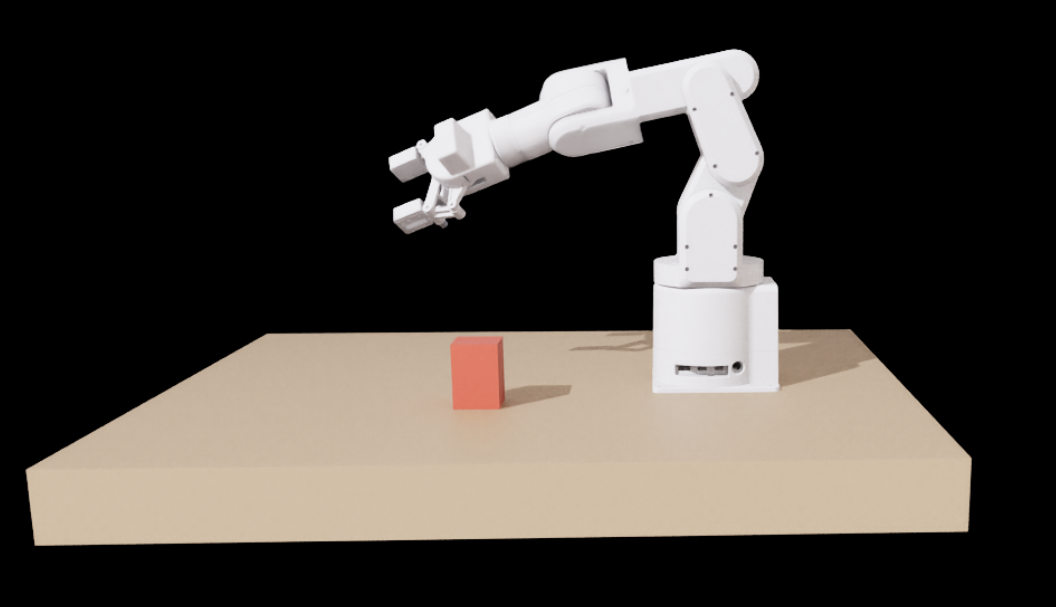
\includegraphics[width=.92\textwidth]{isaac_scene.png}
\caption{Actual Isaac Sim mechArm scene with table and fixed target object}\label{fig:scene}
\end{figure}

\section{System Architecture and Development Environment}
\subsection{Software and Hardware Configuration}
\begin{table}[H]\centering\caption{Implemented environment}\label{tab:environment}
\begin{tabularx}{\textwidth}{p{3.4cm}Y}
\toprule Item & Actual configuration\\\midrule
Simulation host & Windows; Isaac Sim 5.1.0 under \path{E:/AIRobotic/isaac-sim}\\
ROS environment & Ubuntu 22.04 user space in Docker; ROS 2 Humble and MoveIt 2\\
Container image & Project-specific \path{mecharm-exp2-ros2:humble}\\
Simulated robot & mechArm 270 Pi, six arm joints, adaptive gripper\\
Model source & Elephant Robotics \path{mycobot_ros2}, Humble branch\cite{elephantrepo}\\
Transport & TCP server in Isaac Sim, port 8765; newline-delimited JSON\\
Physics/update rate & Isaac physics 120 Hz; render 60 Hz; ROS/TCP state and targets 120 Hz\\
Physical platform & DJI RoboMaster EP, firmware 01.01.1150\\
Physical control host & Windows PowerShell, Conda \path{robomaster}, Python 3.8\\
Physical SDK & RoboMaster SDK 0.1.1.68, AP Wi-Fi, TCP protocol\\
Version control & Public GitHub repository, main branch, 31 commits at report generation\\
\bottomrule
\end{tabularx}
\end{table}

\subsection{Why a TCP Adapter Was Used}
An early topology placed ROS 2 nodes in WSL and Isaac Sim on Windows. Proxy TUN routing and DDS multicast discovery produced inconsistent outcomes: ROS 2 nodes could discover each other locally or Isaac could communicate across systems, but both were not reliable at the same time. A Fast DDS discovery-server trial also failed to expose \path{/joint_states} consistently. The final design isolates all ROS 2 participants inside one Docker network/process environment and replaces cross-system DDS with a narrow TCP adapter. This is a transport change, not a change to the task's joint-state semantics.

\begin{figure}[H]\centering
\begin{tikzpicture}[node distance=8mm,box/.style={draw=black,rounded corners=1pt,minimum height=10mm,text width=3.2cm,align=center,font=\small},arrow/.style={-Latex,thick}]
\node[box](task){ROS 2 task node\\numerical IK and state machine};
\node[box,right=of task](ros){ROS 2 TCP bridge\\joint targets and states};
\node[box,right=of ros](tcp){TCP 8765\\newline JSON};
\node[box,right=of tcp](isaac){Isaac Sim 5.1\\PhysX articulation};
\node[box,below=10mm of task](cfg){YAML parameters\\A, B, heights, gripper};
\node[box,below=10mm of isaac](scene){USD scene\\robot, table, object};
\draw[arrow](cfg)--(task);\draw[arrow](task)-- node[above,font=\scriptsize]{\path{/mecharm/joint_target}}(ros);
\draw[arrow](ros)--(tcp);\draw[arrow](tcp)--(isaac);\draw[arrow](isaac)--(scene);
\draw[arrow,bend left=25](isaac) to node[below,font=\scriptsize]{measured joint state}(tcp);
\draw[arrow,bend left=25](tcp) to (ros);\draw[arrow,bend left=25](ros) to node[below,font=\scriptsize]{\path{/joint_states}}(task);
\end{tikzpicture}
\caption{Final simulation control topology}\label{fig:architecture}
\end{figure}

\subsection{Repository Organization}
The main functional boundaries are:
\begin{table}[H]\centering\caption{Experiment-two repository structure}
\begin{tabularx}{\textwidth}{p{4.5cm}Y}\toprule Path & Responsibility\\\midrule
\path{simulation/isaac/} & Isaac startup, scene generation, TCP joint server, grasp monitor\\
\path{simulation/urdf/} & Official robot/gripper URDF and mesh assets with license\\
\path{src/mecharm_pick_place/} & ROS 2 task, IK, smooth execution, recorder, Launch files, tests\\
\path{src/mecharm_moveit_config/} & SRDF, kinematics, controllers, OMPL, RViz configuration\\
\path{config/} & Simulation, bridge, controller, task, A/B, and height parameters\\
\path{scripts/} & Windows startup, firewall, and Isaac helpers\\
\path{robomaster_ep/} & Physical RoboMaster EP connection, motion, camera, and retry scripts\\
\path{docs/videos/} & Successful simulation, simulation failure, and physical demonstration recordings\\
\path{results/simulation/} & Recorder output locations and parameter snapshots\\
\bottomrule\end{tabularx}
\end{table}

\section{Simulation Scene and Adaptive-Gripper Model}
\subsection{Official Model Import}
The mechArm 270 Pi and adaptive-gripper files were copied from the official Elephant Robotics ROS 2 repository's Humble branch. The checked-in license is retained under \path{simulation/urdf/mycobot_description/LICENSE}. Isaac's URDF importer receives an ASCII-only temporary copy because the 5.1 importer could not reliably parse the Chinese project path. The imported base is fixed, collision geometry is generated from visual meshes, and selective self-collision is enabled.

The final scene contains a fixed-base arm, table, red target block, lighting, camera views, and a physics scene. In the direct Cartesian experiment, the object starts at point A. Odd cycles transfer A to B and even cycles transfer B back to A, allowing one object to support five continuous attempts without resetting the scene.

\subsection{Closed-Loop Gripper Repair}
The adaptive gripper is a four-bar mechanism. A conventional URDF is a tree, so the official model does not encode the two distal joints that close the left and right linkage loops. The mesh files also include pivot holes but no separate bolt/pin geometry. Importing this representation directly allowed the inner links to move without reliably carrying the outer jaws, which appeared as loose or collapsed fingers.

The implemented repair has four parts:
\begin{enumerate}
\item remove all drive attributes from the two outer jaw joints so they are truly passive;
\item add left and right PhysX revolute loop joints between the inner linkage and outer jaw;
\item place the loop constraints outside the tree articulation with \texttt{excludeFromArticulation=true};
\item create four non-colliding cylindrical pins for visual completeness while leaving the revolute joints as the physical constraints.
\end{enumerate}
The articulation solver uses 64 position iterations and 64 velocity iterations. This reduces visible separation at the pin holes under load. Figure~\ref{fig:holes} shows point-cloud projections used to locate the mesh holes rather than estimating pin coordinates by eye.

\begin{figure}[H]\centering
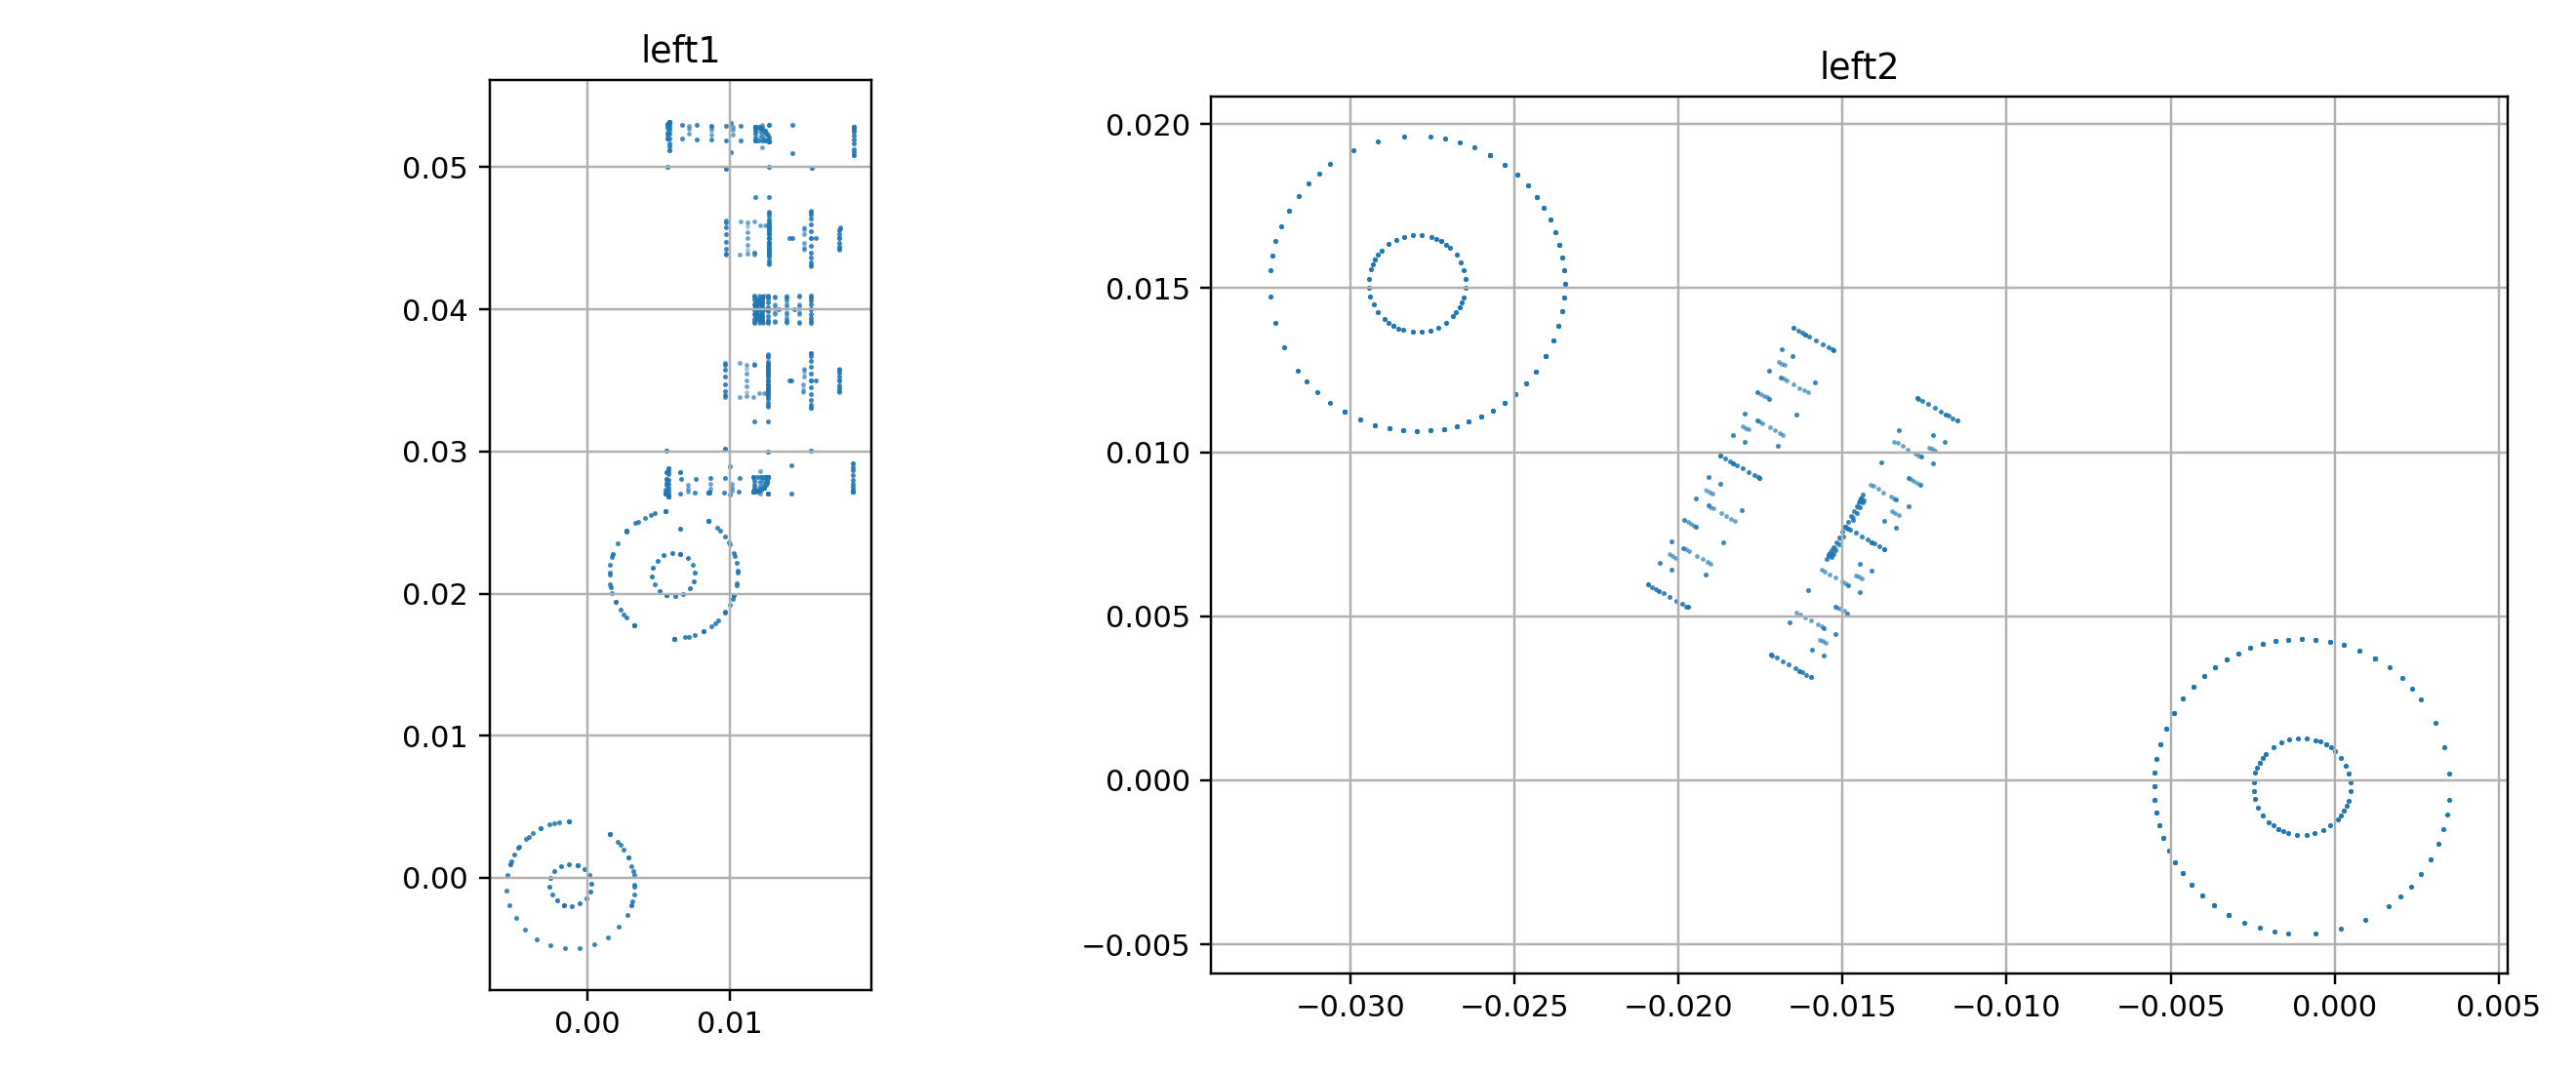
\includegraphics[width=.96\textwidth]{gripper_hole_projection_scene.png}
\caption{Projected gripper mesh geometry used to identify linkage pivot holes}\label{fig:holes}
\end{figure}

\subsection{Mimic Replacement and Drive Tuning}
PhysX 5.1 did not reliably execute several mimic followers of the same reference joint: one gripper side could be ignored without a hard failure. The scene therefore imports with \texttt{parse\_mimic=False}. The master, left inner link, and two right inner links receive explicit angular drives. The TCP bridge mirrors the scalar gripper command as
\begin{equation}
q_{L2}=q_g,\qquad q_{R2}=q_{R3}=-q_g.
\end{equation}
The outer jaws are not commanded; they follow through the physical loop constraints. The current imported-arm defaults are drive strength 1000 and position-drive damping 30000. Commanded gripper joints use stiffness 150, damping 60, and maximum force 10. These are the checked-in final tuning values, not universal manufacturer parameters.

Selective self-collision filters adjacent arm links, overlapping arm/gripper meshes, and internal gripper pairs. Collision between the two final opposing jaws remains enabled. This retains the contact relevant to grasping while preventing imported mesh overlap from destabilizing the articulation.

\subsection{Object Retention Model and Fidelity Limit}
At each physics step, the grasp monitor checks the master gripper position and the gripper-to-object distance. When $q_g\leq-0.68$ rad and the distance is no more than 0.08 m, it creates a PhysX fixed joint between the gripper body and the target. When $q_g\geq0.08$ rad, it removes the joint. This makes transport repeatable for a systems-integration experiment, but it is not a pure friction/contact grasp model. The successful transfer therefore verifies kinematics, sequencing, transport, and release logic more strongly than contact-force realism.

\section{Kinematics, Trajectory Generation, and Task Logic}
\subsection{Fixed Cartesian Targets}
The final parameters in \path{direct_cartesian_pick_place.yaml} are listed in Table~\ref{tab:parameters}. The target-object center has $z=0.025$ m and the cube top is approximately $z=0.050$ m. The pre-grasp tool target is therefore $z=0.125$ m. The closing target is $z=0.065$ m, leaving clearance above the object before the fingers close.
\begin{table}[H]\centering\caption{Final direct Cartesian parameters}\label{tab:parameters}
\begin{tabular}{lll}\toprule Parameter & Value & Meaning\\\midrule
\path{pick_xyz} & $[0.18,0.09,0.025]$ m & Point A/object center\\
\path{place_xyz} & $[0.18,-0.08,0.025]$ m & Point B/object center\\
\path{pregrasp_clearance} & 0.10 m & Approach/lift/retreat clearance\\
\path{pick_close_clearance} & 0.04 m & Height increment at close/release\\
\path{grasp_yaw_offset_deg} & $90^{\circ}$ & In-plane rotation relative to HOME tool axis\\
\path{position_tolerance} & 0.008 m & Numerical IK position tolerance\\
\path{vertical_axis_dot_min} & 0.975 & Minimum vertical alignment score\\
\path{gripper_open} & 0.15 rad & Open target\\
\path{gripper_closed} & $-0.75$ rad & Closed target\\
\path{gripper_speed_rad_s} & 0.12 rad/s & Open/close speed\\
Wait before/after gripper & 1.0/1.5 s & Settling around contact events\\
\bottomrule\end{tabular}
\end{table}

\subsection{Numerical Inverse Kinematics}
The URDF-based solver computes forward kinematics for six arm joints and uses nonlinear least squares from several seeds. Its objective combines Cartesian position and end-effector orientation. If $\mathbf{z}_t$ is the required downward tool axis and $\mathbf{z}(\mathbf{q})$ the actual normalized axis, the orientation condition is represented by
\begin{equation}
d=\mathbf{z}_t^{\mathsf{T}}\mathbf{z}(\mathbf{q}),\qquad d\geq0.975.
\end{equation}
The in-plane tool direction is computed from the HOME pose and rotated by $90^{\circ}$ only during grasp-related Cartesian solving. It does not alter the stored HOME joint vector. A solution is rejected when position error, vertical alignment, finite-value, or joint-limit checks fail. The explicit error includes the best position error and axis dot product, which made the earlier ``only joint 6 moves'' and tilted-tool faults diagnosable.

\subsection{Quintic S-Curve and Speed Separation}
Direct joint execution interpolates each segment with the quintic smoothstep
\begin{equation}
s(u)=6u^5-15u^4+10u^3,\qquad u\in[0,1],
\end{equation}
and sends
\begin{equation}
\mathbf{q}(u)=\mathbf{q}_0+s(u)(\mathbf{q}_1-\mathbf{q}_0)
\end{equation}
at 120 Hz. Because $\max(ds/du)=1.875$, segment duration is computed using the desired peak-speed limit divided by 1.875. The current source uses 28 deg/s for normal repositioning and 4 deg/s for the vertical stages \texttt{PICK\_GRASP}, \texttt{LIFT}, \texttt{PLACE\_GRASP}, and \texttt{RETREAT}. The gripper is slower at 0.12 rad/s in the Cartesian flow. This separation retains practical transfer speed while reducing excitation near the object and table.

Feedback pacing prevents large catch-up jumps. Scheduling gaps are capped at two target periods; progress pauses when fresh feedback is unavailable; feedback older than 5 s raises \texttt{DIRECT\_MOTION\_FEEDBACK\_TIMEOUT} and holds the last target.

\subsection{Alternating Five-Cycle State Sequence}
\begin{figure}[H]\centering
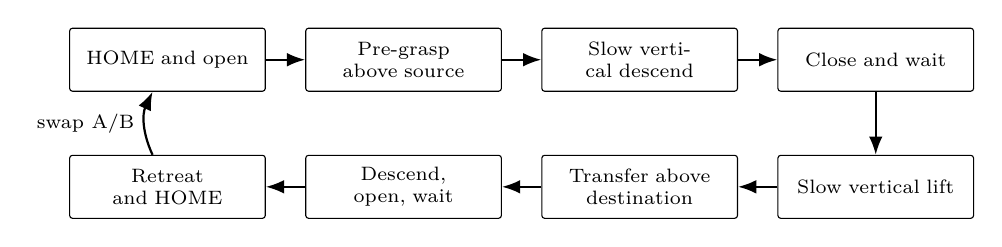
\begin{tikzpicture}[node distance=5mm,box/.style={draw=black,rounded corners=1pt,minimum height=8mm,text width=2.25cm,align=center,font=\scriptsize},arrow/.style={-Latex,thick}]
\node[box](home){HOME and open};
\node[box,right=of home](pa){Pre-grasp above source};
\node[box,right=of pa](down){Slow vertical descend};
\node[box,right=of down](close){Close and wait};
\node[box,below=8mm of close](lift){Slow vertical lift};
\node[box,left=of lift](transfer){Transfer above destination};
\node[box,left=of transfer](release){Descend, open, wait};
\node[box,left=of release](return){Retreat and HOME};
\draw[arrow](home)--(pa);\draw[arrow](pa)--(down);\draw[arrow](down)--(close);
\draw[arrow](close)--(lift);\draw[arrow](lift)--(transfer);\draw[arrow](transfer)--(release);\draw[arrow](release)--(return);
\draw[arrow,bend left=25](return) to node[left,font=\scriptsize]{swap A/B}(home);
\end{tikzpicture}
\caption{One alternating grasp cycle}\label{fig:sequence}
\end{figure}
The node opens the gripper, moves to HOME, calculates the grasp tool axis, and runs the sequence in Figure~\ref{fig:sequence}. For odd cycles, source/destination are A/B; for even cycles they are B/A. Every cycle returns to HOME before the next begins. The default Launch argument is \texttt{cycles:=5}.

\section{ROS 2 Nodes, Launch Files, and Recording}
\subsection{Main Nodes and Interfaces}
\begin{table}[H]\centering\caption{ROS 2 nodes and interfaces}
\begin{tabularx}{\textwidth}{p{4.0cm}p{4.0cm}Y}\toprule Component & Interface & Function\\\midrule
Cartesian task & subscribes \path{/joint_states}; publishes \path{/mecharm/joint_target} & IK, state sequence, smooth targets\\
Container TCP bridge & same two ROS topics & Converts JointState messages to/from TCP JSON\\
Isaac TCP server & TCP 8765 & Applies targets to PhysX and returns measured positions\\
Trajectory controller & \path{/mecharm_controller/follow_joint_trajectory} & Standard action-compatible streamed execution\\
Recorder & status/result/joint topics & Writes events, summaries, errors, and trajectory CSV\\
\bottomrule\end{tabularx}
\end{table}
The MoveIt 2 configuration, RViz display, OMPL pipeline, and \texttt{FollowJointTrajectory} controller remain available. During development, RViz successfully displayed the robot after DDS discovery was corrected. The final five-cycle demonstration uses the direct numerical-IK path because the imported collision geometry and planning-scene calibration were not yet accurate enough for reliable OMPL execution.

\subsection{Launch Entry Points}
The main experiment entry points are:
\begin{itemize}
\item \path{cartesian_direct_pick_place.launch.py}: one A-to-B cycle;
\item \path{alternating_cartesian_pick_place.launch.py}: five alternating cycles;
\item \path{empty_grasp_test.launch.py}: empty-point exception and HOME return;
\item \path{simulation_moveit.launch.py}: MoveIt/RViz integration path.
\end{itemize}
The alternating Launch starts the ROS-side TCP bridge and, after a 2 s delay, the Cartesian task. Isaac Sim is an independent simulator process, so starting it separately does not reduce the completeness of the ROS 2 Launch entry point.

\subsection{Result Recorder and Evidence Gap}
The recorder can create a timestamped directory containing \path{events.jsonl}, \path{summary.csv}, \path{trajectory.csv}, \path{errors.log}, and a copied parameter snapshot. For this fixed-point experiment, the authoritative trajectory is the finite waypoint sequence stored in the source and YAML configuration, so the same motion can be reproduced without reconstructing it from a sampled stream. Execution results, exception outputs, parameters, and videos are preserved in the final evidence package. The recorder remains available when a raw time-series trace is desired, but it is not required to define the fixed trajectory.

\section{Error Handling and Safety Behavior}
\subsection{Simulation Faults}
\begin{table}[H]\centering\caption{Implemented simulation fault behavior}\label{tab:faults}
\begin{tabularx}{\textwidth}{p{4.0cm}p{4.2cm}Y}\toprule Fault & Detection & Safe behavior\\\midrule
No joint state & 5--8 s startup deadline & Emit \texttt{NO\_JOINT\_STATE}; do not begin motion\\
Invalid joint state & Missing/non-finite values & Reject input; no target is generated\\
Unreachable/no IK & Least-squares result violates tolerance or alignment & Emit \texttt{NUMERIC\_IK\_FAILED}; stop task\\
Stale feedback & No new state for more than 5 s during direct motion & Hold last target and raise timeout\\
Empty grasp test & Deliberate close at known empty B in a fresh scene & Emit \texttt{NO\_OBJECT}, reopen, retreat, HOME\\
Joint limit & URDF numerical bounds and controller validation & Reject solution or abort execution\\
\bottomrule\end{tabularx}
\end{table}
The empty-grasp program is a controlled exception test, not sensor-based object detection. It uses a known empty point, closes the gripper, emits a deterministic error, and returns to HOME. The project does not claim that the simulation can infer grasp success from contact force.

\subsection{Physical-Robot Safety}
The RoboMaster EP retry program requires an operator confirmation before movement. It parks the arm at $(x,y)=(0,150)$ mm before chassis rotation, moves to $(220,0)$ mm only at the grasp side, uses chassis angular speed 30, and gripper power 50. A background keyboard monitor accepts the E key, stops the chassis, pauses the gripper, and prevents later commands. Cleanup stops camera streaming, unsubscribes gripper status, stops active mechanisms, and closes the SDK connection.

Gripper \texttt{closed} status alone cannot prove that an object is held. The retry script therefore measures closing time: below 1.85 s is treated as a likely object contact, while 1.85 s or longer is treated as empty and triggers a return to the cycle's safe start direction. This is an empirical heuristic, not calibrated force sensing. A timeout of 5 s exits safely when no closed status arrives.

\section{Simulation Build, Tests, and Recorded Results}
\subsection{Build and Transport Validation}
The experiment-specific Docker build completed and the workspace build reported four finished packages: \path{mycobot_description}, \path{mecharm_moveit_demo}, \path{mecharm_pick_place}, and \path{mecharm_moveit_config}. A direct transport probe produced the following terminal sequence:
\begin{lstlisting}[caption={Observed direct-motion transport result}]
MOTION_PROBE_OUTBOUND
MOTION_PROBE_RETURN
MOTION_PROBE_SUCCESS
\end{lstlisting}
This confirmed that the ROS target crossed the container/Windows boundary, Isaac moved the articulation, and the measured state returned to ROS 2.

\subsection{Successful Five-Cycle Simulation}
The final successful recording is {\reportcjk\small docs/videos/仿真连续五次抓取.mp4}. Programmatic metadata extraction measured 385.57 s, 30.002 FPS, and 11,568 frames. The recording shows the Isaac scene and running terminal throughout the alternating A-to-B/B-to-A sequence. The project video index explicitly identifies it as a successful five-cycle run. Representative frames appear in Figure~\ref{fig:simfive}.
\begin{figure}[H]\centering
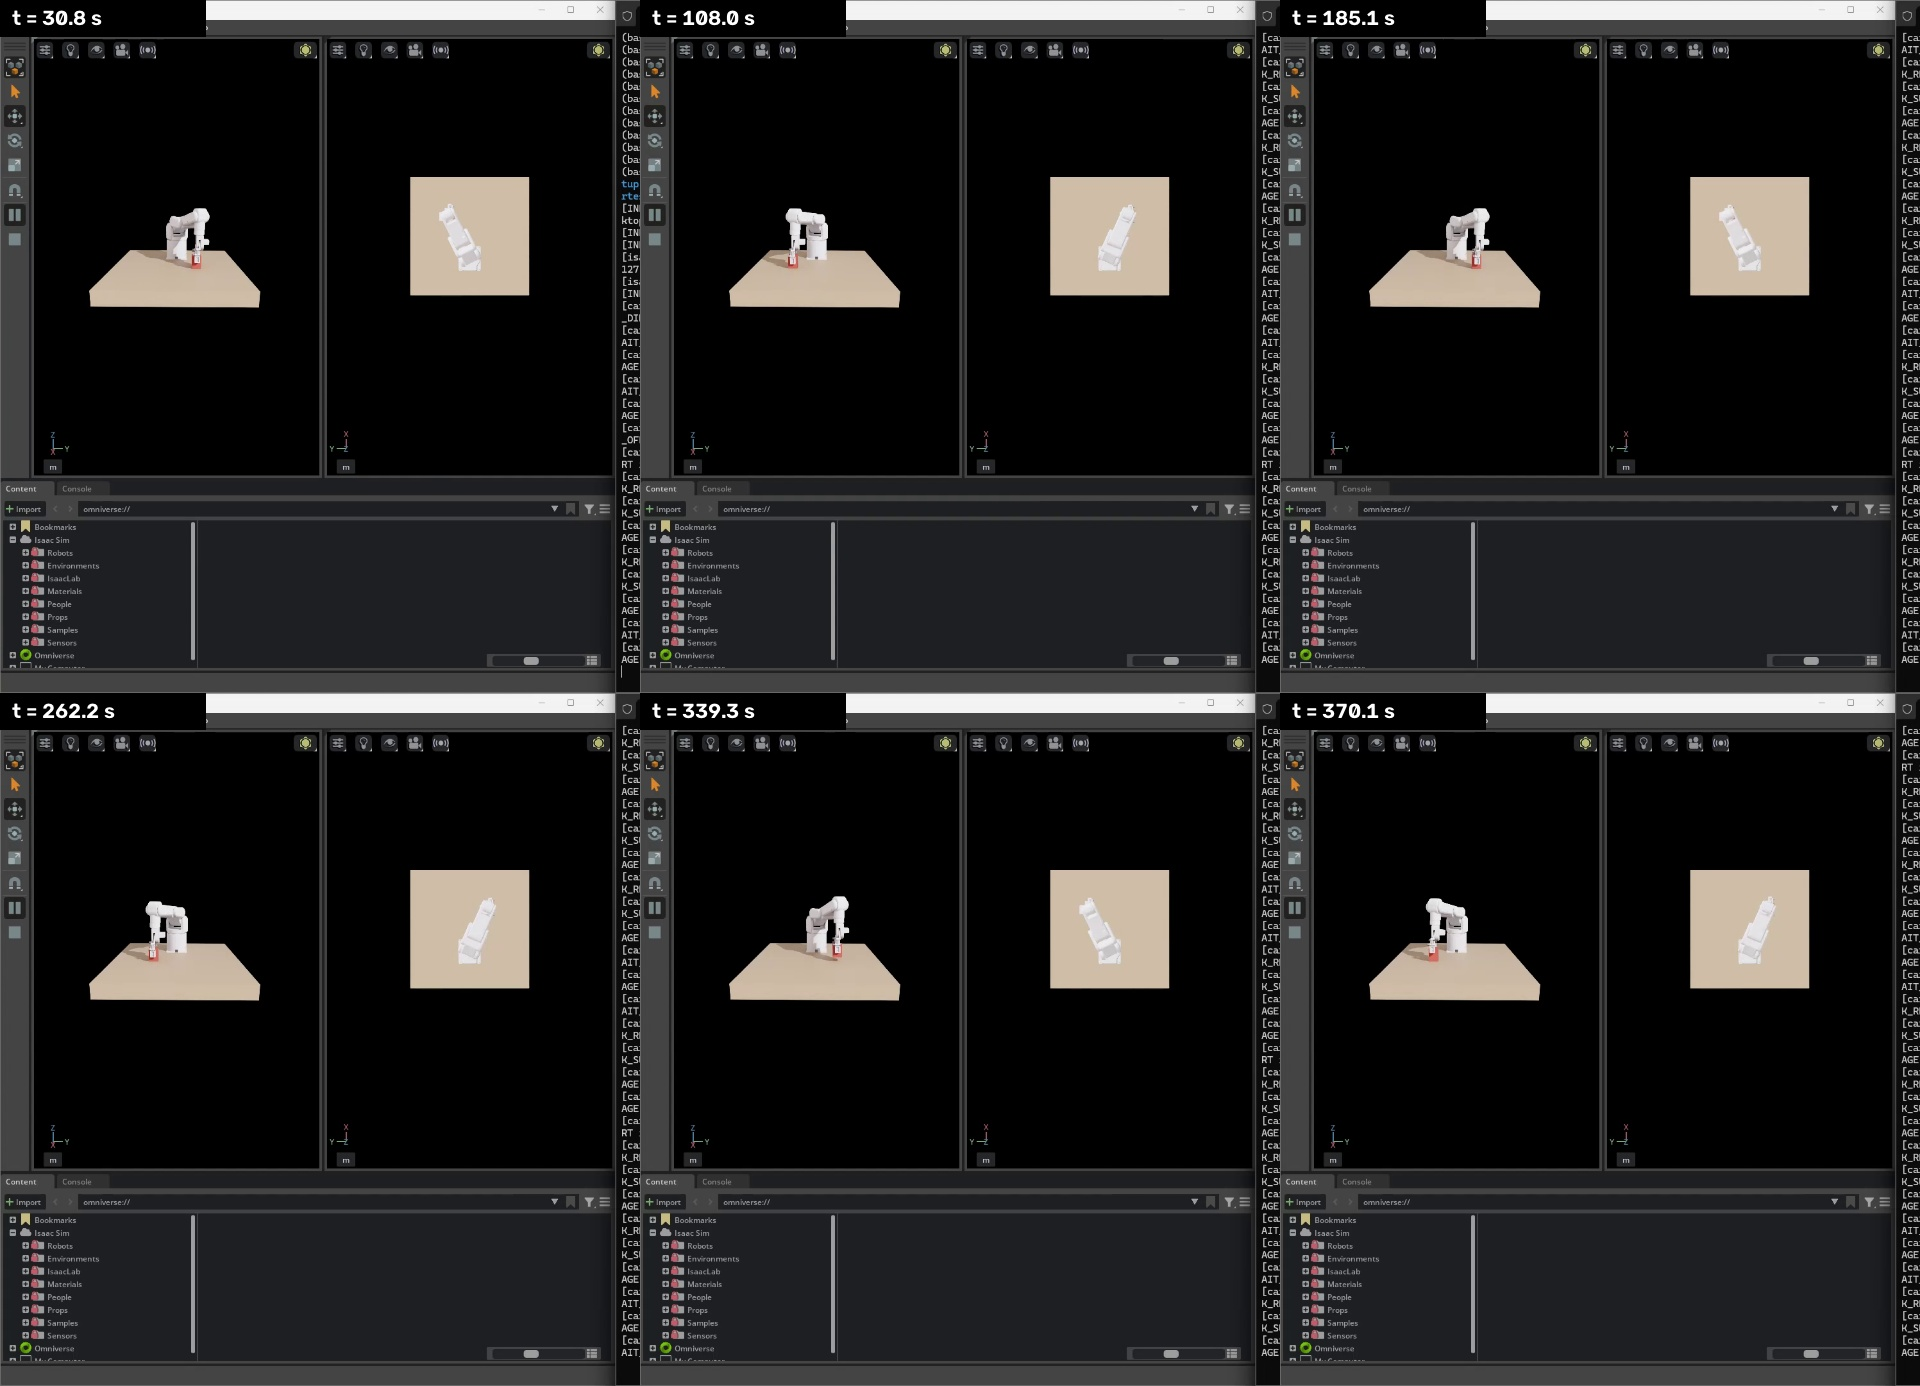
\includegraphics[width=.92\textwidth]{simulation_five_cycle_contact_sheet.jpg}
\caption{Representative frames from the recorded successful five-cycle simulation}\label{fig:simfive}
\end{figure}

\subsection{Preserved Failure Case}
The separate file {\reportcjk\small docs/videos/仿真连续五次抓取（失败案例）.mp4} is 54.06 s at 30.004 FPS (1,622 frames). It preserves a failed run rather than replacing it with a successful replay. Figure~\ref{fig:simfail} shows the arm progressing through the attempted approach and returning/stopping without transferring the block. Together with explicit numerical-IK logging, this provides qualitative evidence of failure visibility, although no paired structured error file was saved.
\begin{figure}[H]\centering
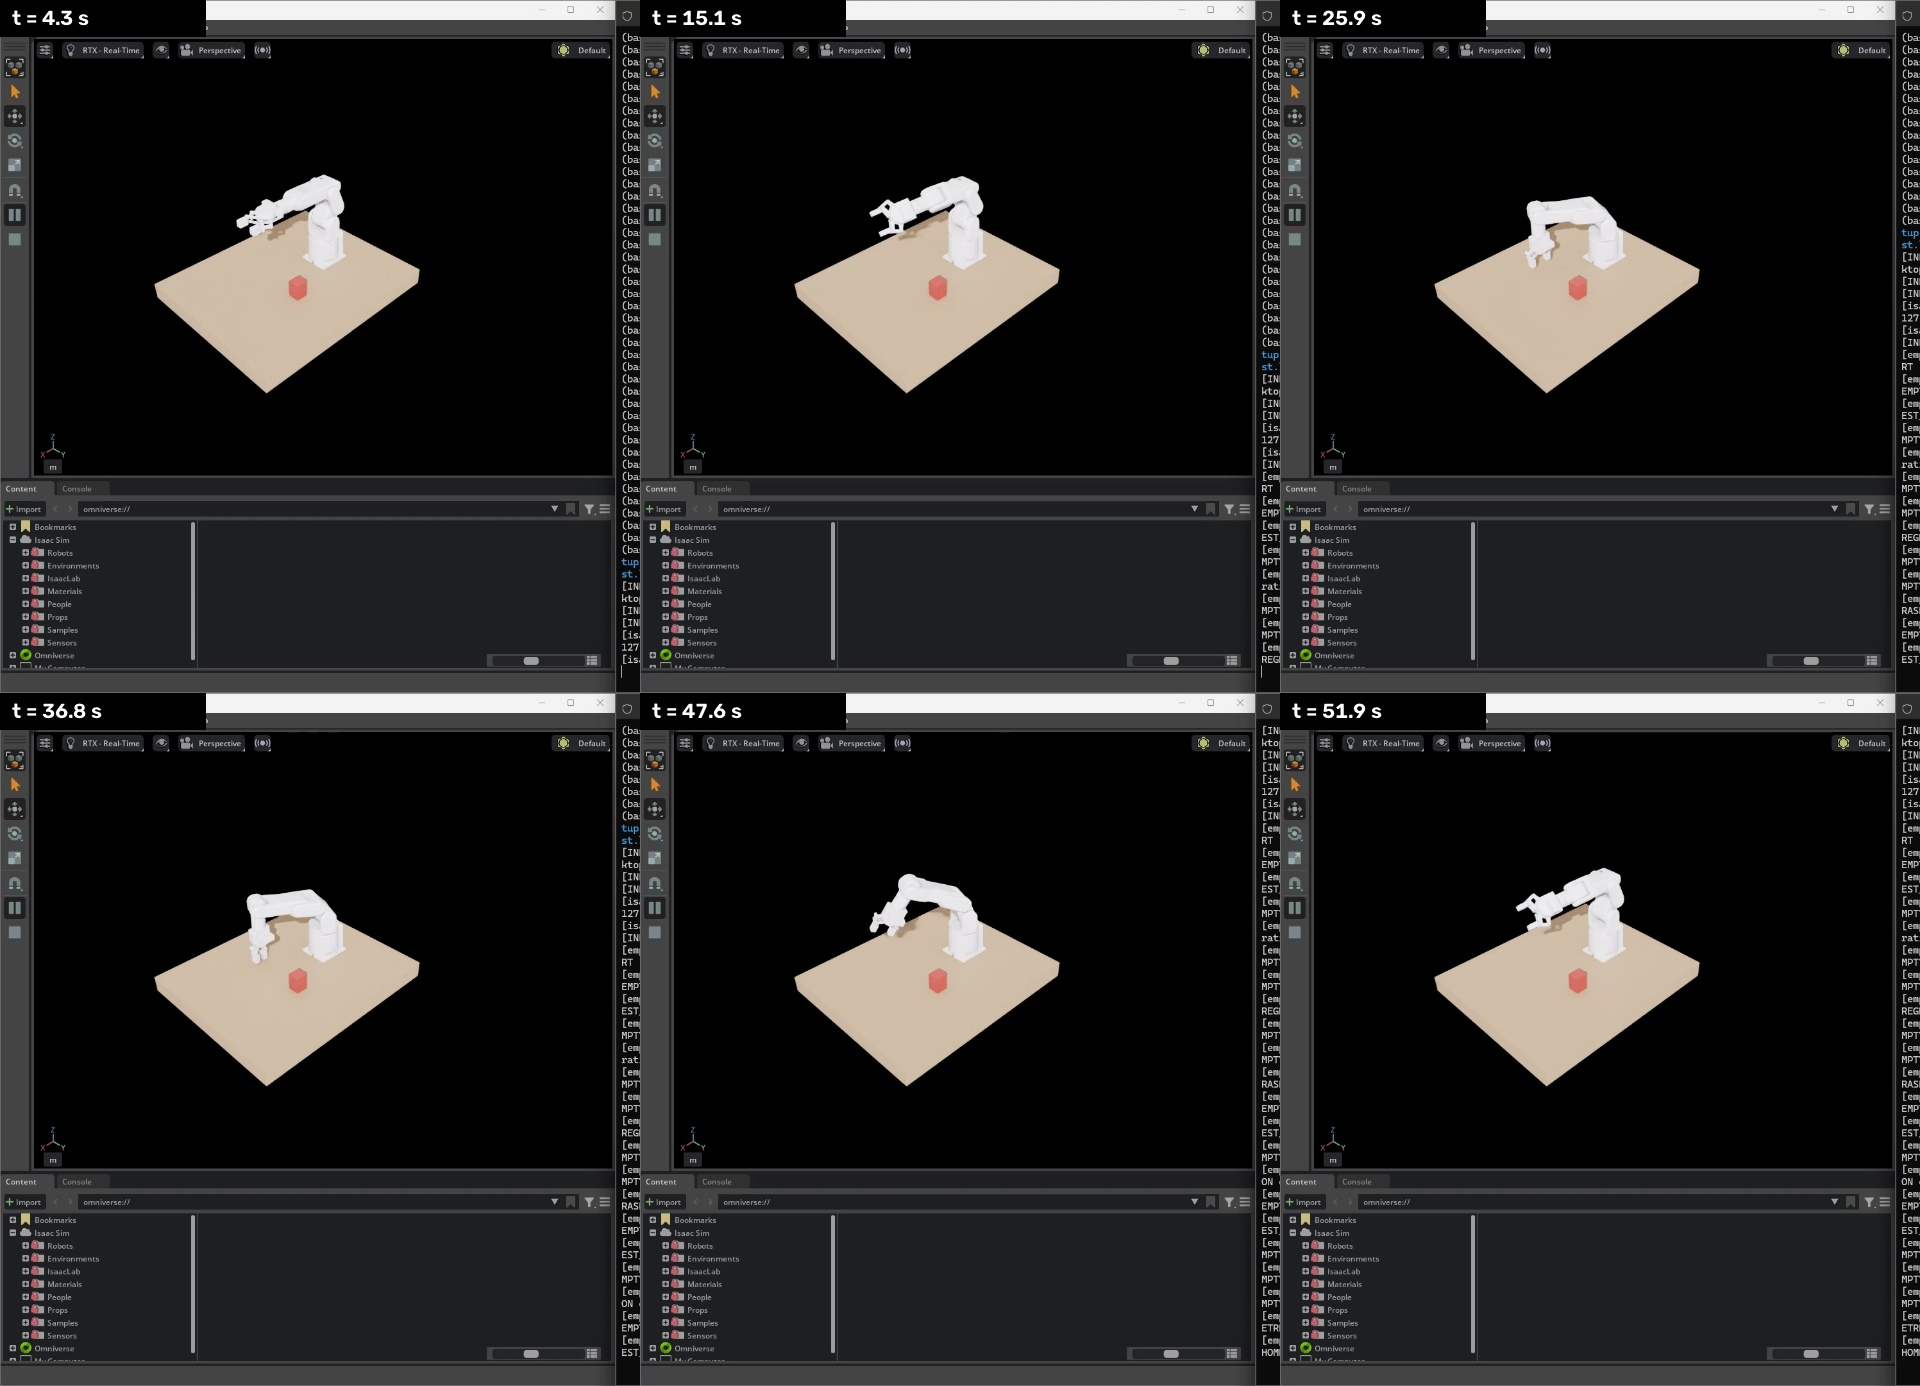
\includegraphics[width=.84\textwidth]{simulation_failure_contact_sheet.jpg}
\caption{Representative frames from the preserved simulation failure recording}\label{fig:simfail}
\end{figure}

\subsection{Current Lightweight Regression Result}
A fresh test run selected only tracked experiment-two tests and excluded unrelated untracked files. It executed 38 tests in 1.56 s: 36 passed and two failed. The failures are contract/source-text assertions rather than runtime simulation failures:
\begin{enumerate}
\item one test still expects the old sequence ``initially close gripper before approach'', while the current required behavior opens at startup and closes only at the object;
\item one test expects vertical speed 8 deg/s, while the checked-in source currently uses 4 deg/s.
\end{enumerate}
These failures identify stale tests that should be updated after the intended parameters are formally frozen. They also mean the repository cannot presently be reported as having a completely passing automated test suite.

\section{Physical Verification on RoboMaster EP}
\subsection{Implemented Physical Sequence}
The physical program uses the RoboMaster EP's planar arm and chassis rotation. Because this robot differs kinematically from the six-axis mechArm, the task is expressed as safe arm positions and chassis yaw:
\begin{enumerate}
\item park at $(0,150)$ mm and open the gripper;
\item rotate the chassis $\pm45^{\circ}$ toward the source;
\item move the arm to $(220,0)$ mm and close;
\item park, rotate $\mp90^{\circ}$ toward the destination, and descend;
\item open, park, rotate $\pm45^{\circ}$ back to the initial direction;
\item reverse all rotation signs on the next cycle.
\end{enumerate}
The simple five-cycle program executes exactly five attempts. The retry version instead counts five successful grasps and repeats a cycle after an inferred empty grasp. It also shows the 360p camera stream and supports E-key interruption.

\subsection{Recorded Hardware Result}
The file {\reportcjk\small docs/videos/真机连续五次抓取（包含失败案例）.mp4} has duration 186.87 s, 30.000 FPS, and 5,606 frames. It visibly records the RoboMaster EP, marked floor workspace, object, arm, gripper, and repeated chassis/arm motion. The recording intentionally includes a failure case. Representative frames in Figure~\ref{fig:hardware} show the robot in safe/parked, approach, transport, and return configurations.
\begin{figure}[H]\centering
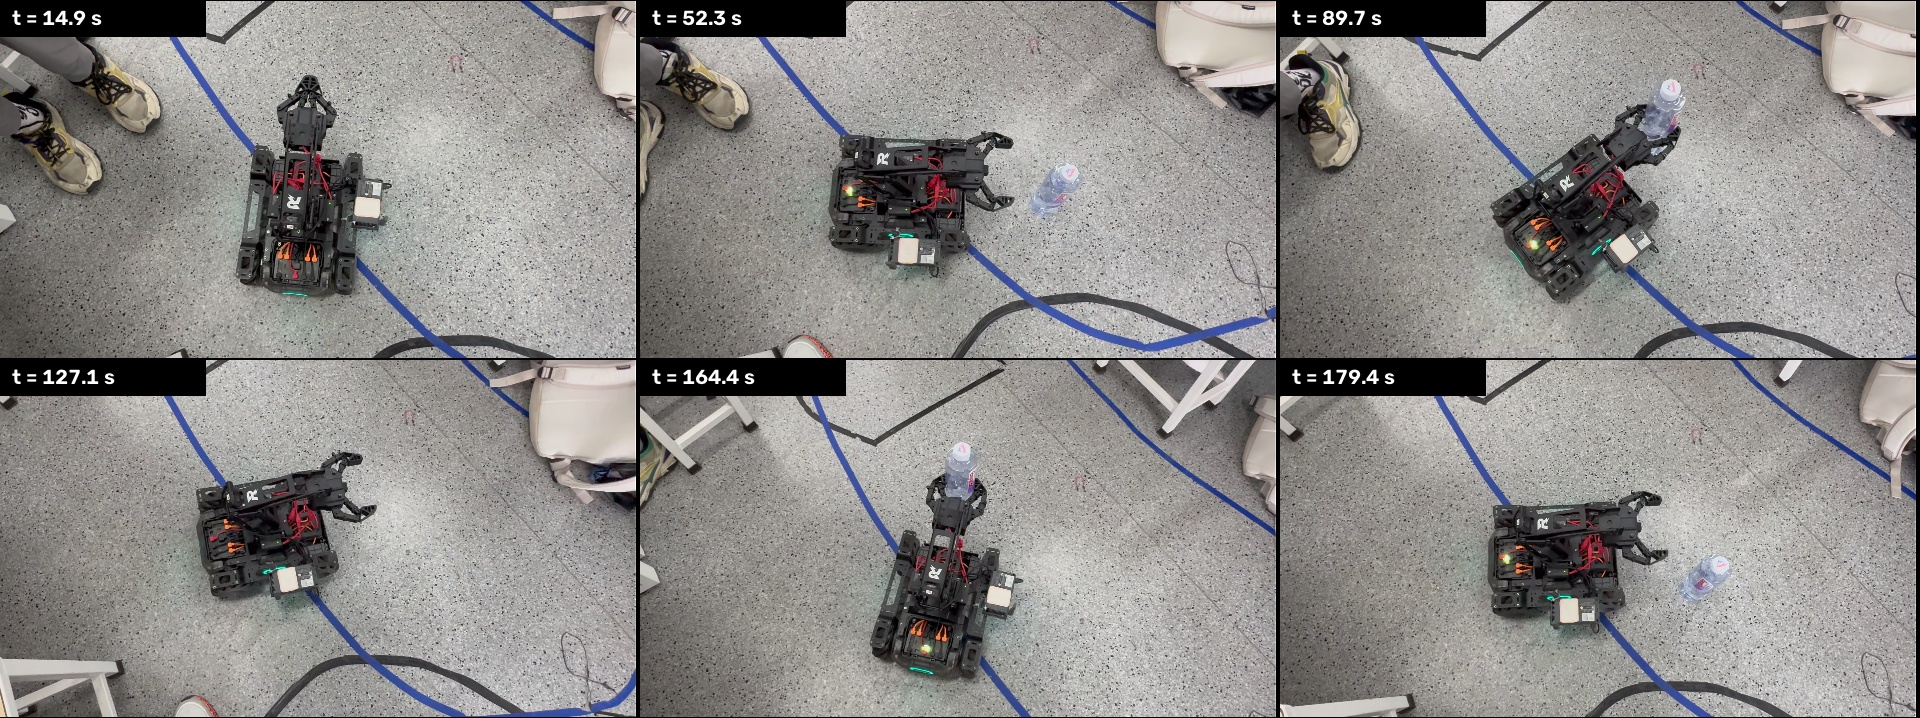
\includegraphics[width=.92\textwidth]{hardware_five_cycle_contact_sheet.jpg}
\caption{Representative frames from the physical RoboMaster EP five-cycle recording}\label{fig:hardware}
\end{figure}

The repository does not contain a timestamped table mapping each physical attempt to success/failure. Therefore the video verifies that the physical sequence was exercised and a failure was preserved, but it does not independently prove the guide's exact ``at least 4 of 5'' count. The report does not infer an unsupported count from the filename alone.

\subsection{Deviation from the Required Physical Platform}
The guide specifies Jetson Orin and mechArm 270 for the physical stage. Those devices were not available for this course run, so the instructor approved DJI RoboMaster EP as the substitute. I completed the physical fixed-point task through the EP's Windows Python SDK. The RoboMaster chassis performed the transfer rotation and its arm has different degrees of freedom and coordinates, so the ROS 2 interface is not identical to simulation. This is an approved equipment adaptation, not an unfinished physical demonstration.

\section{Reproducibility and Operating Procedure}
\subsection{Simulation Startup}
From Windows PowerShell, the checked-in workflow is:
\begin{lstlisting}[caption={Build and start the simulation runtime}]
cd "E:\机器人集成小组项目\实验二"
.\scripts\start_moveit_sim.ps1

docker compose -f ".\docker-compose.yml" exec moveit bash -lc \
 "source /opt/ros/humble/setup.bash && \
  colcon --log-base /opt/mecharm_ws/log build \
  --base-paths /workspace/mecharm_exp2/simulation/urdf/mycobot_description \
  /workspace/mecharm_exp2/src \
  --build-base /opt/mecharm_ws/build \
  --install-base /opt/mecharm_ws/install --symlink-install"
\end{lstlisting}
After the Isaac timeline is playing and the TCP server is listening, the five-cycle task is:
\begin{lstlisting}[caption={Run five alternating simulation cycles}]
docker compose exec moveit bash -lc \
 "source /opt/ros/humble/setup.bash && \
  source /opt/mecharm_ws/install/setup.bash && \
  ros2 launch mecharm_pick_place \
  alternating_cartesian_pick_place.launch.py \
  project_root:=/workspace/mecharm_exp2 cycles:=5"
\end{lstlisting}
The empty-grasp exception is launched by replacing the Launch filename with \path{empty_grasp_test.launch.py}. The expected terminal evidence is \texttt{EMPTY\_GRASP\_EXCEPTION code=NO\_OBJECT} followed by \texttt{EMPTY\_GRASP\_RETURN\_HOME}.

\subsection{Physical-Robot Startup}
The physical computer must first connect directly to the RoboMaster EP Wi-Fi. Then:
\begin{lstlisting}[caption={Prepare the verified RoboMaster SDK environment}]
conda activate robomaster
$env:RM_SDK_ROOT = "C:\Users\xhr\RoboMaster-SDK-fixed"
python -c "import os; root=os.environ['RM_SDK_ROOT']; \
keep=[os.add_dll_directory(os.path.join(root,'lib','libmedia_codec', \
'src','ffmpeg-dll')), os.add_dll_directory(os.path.join(root,'lib', \
'libmedia_codec','src','opus-dll'))]; exec(open( \
r'E:\机器人集成小组项目\实验二\robomaster_ep\scripts\ \
pick_rotate_place_5_cycles_retry.py',encoding='utf-8').read())"
\end{lstlisting}
Connection, small arm motion, gripper, chassis rotation, and camera tests should be run before the combined sequence. The motion script must not be run while another device controls the same robot.

\subsection{Version-Control Evidence}
The public repository is \githuburl. At report generation, \path{main} contains 31 commits. Representative milestones include initial documentation, ROS 2 task and Isaac integration, official adaptive-gripper assets, motion stabilization, MoveIt 2 configuration, TCP runtime, Cartesian IK, gripper loop repair, pre-grasp clearance tuning, RoboMaster scripts, retry/five-cycle programs, recordings, and bilingual README updates. Videos are managed through Git LFS because two files exceed GitHub's normal 100 MB file limit.

\begin{longtable}{p{2.0cm}p{4.0cm}p{7.0cm}}
\caption{Representative incremental commits}\\\toprule Commit & Type & Content\\\midrule\endfirsthead
\toprule Commit & Type & Content\\\midrule\endhead
a25b4b2 & feat & ROS 2 task and Isaac Sim integration\\
377ab33 & feat & Official mechArm adaptive-gripper assets\\
4739d15 & feat & Stable Isaac scene integration\\
5fb030b & feat & MoveIt 2 configuration\\
fd7be61 & fix & End-to-end trajectory transport\\
0026efe & feat & Containerized TCP runtime\\
c5863e9 & feat & Calibrated Cartesian grasping\\
8220502 & fix & Adaptive-gripper loop physics and scene refresh\\
ac41e48 & tune & Higher pre-grasp clearance\\
5140448 & tune & Grasp pose and Isaac drive parameters\\
4e6f3d2 & feat & Physical retry and multi-cycle scripts\\
50f8de2 & feat & Alternating tests and experiment recordings\\
324ea5f & docs & Chinese and English operating instructions\\
\bottomrule
\end{longtable}

\section{Discussion of Problems and Engineering Decisions}
\subsection{Problems Solved}
The largest integration problems were not the high-level pick/place states but mismatches between model topology, middleware discovery, and dynamic control:
\begin{itemize}
\item The URDF omitted closed-loop gripper constraints, so the distal linkages were repaired with explicit PhysX joints.
\item Multi-follower mimic behavior was unreliable, so the scalar command is mirrored at the transport boundary.
\item Cross-system DDS discovery was unstable under TUN routing, so a dedicated TCP channel replaced it while ROS 2 remained inside the container.
\item Cubic/direct target changes excited visible oscillation, so targets now use a quintic S-curve with separate slow vertical motion.
\item The tool initially approached at an incorrect yaw/tilt, so the numerical solver now preserves verticality and applies yaw relative to the HOME tool axis only during grasping.
\item The gripper descended into the block before closure, so closing height was raised above the object top and open/close settling waits were added.
\end{itemize}

\subsection{Remaining Risks and Limitations}
The main remaining simulation risks are inaccurate collision meshes, the fixed-joint grasp helper, and stale automated contracts. MoveIt/OMPL assets exist, but the recorded five-cycle success uses direct numerical IK rather than collision-aware planning. The fixed trajectory, execution outcomes, parameters, and errors are preserved in the delivery package. A duplicated \path{grasp_yaw_offset_deg} key also exists in the YAML file; both values are currently identical, but the duplicate should be removed to avoid ambiguous future edits.

The physical stage has the larger compliance gap. RoboMaster EP proves that the group operated a real mechanism and handled retries/safe exit, but it cannot validate the mechArm model, six-joint IK, ROS 2 controller, or simulation-to-hardware parameter-only switch. The close-time heuristic can confuse varying object width, friction, battery voltage, or stalled motion with successful grasping. A compliant revision should use physical mechArm feedback, a ROS 2 driver, explicit emergency-stop evidence, and machine-readable attempt logs.

\section{Conclusions and Recommended Completion Work}
The experiment produced a functioning fixed-point simulation with a mechArm 270 Pi model, adaptive-gripper physics repair, fixed A/B points, safe approach/closing heights, vertical numerical IK, a $90^{\circ}$ grasp-yaw offset, quintic 120 Hz joint interpolation, separate normal/vertical speeds, and explicit error handling. A 385.57 s video records five successful alternating cycles, and a separate failure recording is retained. The ROS 2/Docker and Windows Isaac integration is reproducible through the checked-in startup scripts and TCP bridge.

Physical work on RoboMaster EP demonstrates repeated real grasp, chassis transfer, release, retry, camera observation, and safe cleanup. The instructor-approved platform substitution was necessary because the specified hardware was unavailable. The resulting task is complete on the available platform, while the different ROS 2/SDK interface remains an explicitly documented compatibility boundary.

The shortest path to complete strict acceptance is:
\begin{enumerate}
\item optionally add the recorder node to the alternating Cartesian Launch when a raw time-series trace is required; the fixed waypoint and result records are already preserved;
\item update the two stale contract tests and rerun the tracked test suite until all tests pass;
\item combine Isaac startup and ROS task launch behind one documented top-level entry, or obtain instructor approval for the current PowerShell-plus-Launch arrangement;
\item if the specified mechArm 270 and Jetson Orin become available later, validate the existing task logic through the corresponding device interface and calibrated position parameters;
\item record object mass, emergency-stop procedure, per-member safety checks, five attempt outcomes, and at least four successful placements.
\end{enumerate}
With these items, the existing software foundation can be converted from a successful mixed-platform prototype into a fully evidenced course acceptance package.

\clearpage
\appendix
\section{Submission File Cross-Reference}
\begin{longtable}{p{5.0cm}p{8.0cm}}
\caption{Required materials and repository paths}\\\toprule Required material & Repository path/evidence\\\midrule\endfirsthead
\toprule Required material & Repository path/evidence\\\midrule\endhead
ROS 2 programs & \path{src/mecharm_pick_place/}, \path{src/mecharm_moveit_demo/}\\
Launch files & \path{src/mecharm_pick_place/launch/} and \path{src/mecharm_moveit_config/launch/}\\
Parameter files & \path{config/simulation.yaml}; \path{src/mecharm_pick_place/config/direct_cartesian_pick_place.yaml}\\
Simulation model & \path{simulation/urdf/mycobot_description/}; \path{simulation/scenes/mecharm_pick_place.usd}\\
Pick/place/safe height & \path{direct_cartesian_pick_place.yaml}\\
Simulation videos & {\reportcjk\small docs/videos/仿真连续五次抓取.mp4}; failure-case video in same folder\\
Physical video & {\reportcjk\small docs/videos/真机连续五次抓取（包含失败案例）.mp4}\\
Physical programs & \path{robomaster_ep/scripts/}\\
Five-attempt result record & Fixed waypoint/result records and successful simulation video; physical video includes a failure and recovery\\
Exception record & Empty-grasp source/log contract and simulation failure video; standalone final error file still missing\\
Operating instructions & \path{README.md}, \path{README_EN.md}, \path{docs/testing.md}, \path{robomaster_ep/README.md}\\
Report & \path{report/main.tex} and compiled PDF\\
\bottomrule
\end{longtable}

\section{Report Evidence Method}
The report was assembled from the laboratory guide, current tracked source/configuration files, Git history, existing result directories, and the three preserved MP4 files. Contact sheets were generated by \path{report/extract_video_frames.py}; the script decodes fixed relative timestamps and writes reproducible JPEG sheets. Video duration, FPS, and frame counts were read from the decoded streams. No result count was inferred where the repository lacked a per-attempt record.

\clearpage\begingroup\sloppy
\begin{thebibliography}{99}\addcontentsline{toc}{section}{References}
\bibitem{guide} Robot Systems Integration Laboratory. Mechanical Arm Fixed-Point Grasping (Group Experiment): Simulation Development and Physical Verification Requirements[S]. 2026.
\bibitem{elephantrepo} Elephant Robotics. mycobot\_ros2: myCobot ROS 2 Package[EB/OL]. Humble branch. \url{https://github.com/elephantrobotics/mycobot_ros2}.
\bibitem{isaacdocs} NVIDIA Corporation. Isaac Sim Documentation, Version 5.1.0[EB/OL]. \url{https://docs.isaacsim.omniverse.nvidia.com/5.1.0/}.
\bibitem{ros2humble} Open Robotics. ROS 2 Humble Documentation[EB/OL]. \url{https://docs.ros.org/en/humble/}.
\bibitem{moveit} PickNik Robotics. MoveIt 2 Documentation: Humble[EB/OL]. \url{https://moveit.picknik.ai/humble/}.
\bibitem{robomaster} DJI. RoboMaster Python SDK Documentation[EB/OL]. \url{https://robomaster-dev.readthedocs.io/}.
\end{thebibliography}\endgroup
\end{document}
